\documentclass[main.tex]{subfiles}

\begin{document}

\section{Matching Algorithms}
The matching problem is solved on the static graph at a certain point in time. One goal for the optimization algorithms is to find the maximum edge-disjoint cycle covering, which can be solved as Min-D-DCC is solved \cite{Man1} \cite{Bir}. The section \ref{bima} discusses this polynomial time algorithm.

In the case that the optimal soultion contains long cycles, the matching problem is to find the maximum edge-disjoint covering with cycles of $\leq$ edges. This problem is NP-Hard and APX-Complete \cite{Bir}. This is desirable because

Both graph algorithms and integer linear programming (ILP) algorithms can be used. Some additional features may be easier to add in the ILP case , which is a common, reliable choice in the field despite being NP-complete; however additional constraints such as desiring small cycles make the problem NP-Hard. Abraham et al. \cite{Abr1} have used ILP in practice for finding kidney exchanges.

\subsection{Matching via Perfect Bipartite Matching}\label{bima}

An algorithm to find perfect weighted matchings in bipartite graph can be used to discover the optimal match in polynomial time \cite{Bir}. The bipartite graph has one side for Offers and one for Requests, thus each (offer=$t_a$, request=$t_b$) pair has two nodes created with edge weight $0$. Next an edge is created between the offer node and every request node for $t_a$ with weight $> 0$. Then a maximum weight perfect matching algorithm can be used.

The positive weight can be used to assign preferences to some (offer, request) pairs over others, perhaps due to user preferences (soft constraints).

The drawback is that long-cycles are possible, and in the dense graph for kidney exchange, very likely. Each user reserves the right to refuse a suggested match, so longer matches are more likely to be rejected, and in the kidney case, require organizing dozens of simultaneous surgeries. However, bounding the match-size results in an NP-hard problem \cite{Bir}.

\subsubsection{Low Acceptance Probability}
In the case that $p < 0.7$, a simple 2-cycle cover will likely perform best. Perhaps following this up with a maximum cycle cover will be good (if the $(>2)$-cycles haven't been ruined).

\subsubsection{Hanging Offers and Requests}
\begin{figure}
  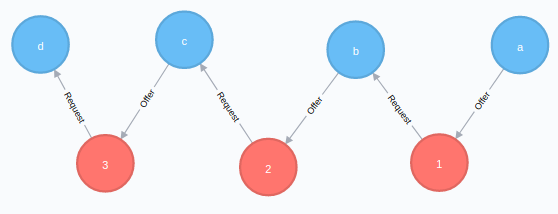
\includegraphics[width=\textwidth]{hanging_example.png}
  \caption{1,2,3 are ORnodes and a,b,c,d are task nodes.}
  \label{hanging_example}
\end{figure}

In the $0.7 < p < 0.95$ range, long cycles will be rejected with high probability. This makes the \ref{bima} scheme infeasible. The Hanging ORnode approach questions whether this is necessessary.

Take the case in Figure \ref{hanging_example}. Assume ORnodes $1,2$ and $3$ are part of a larger cycle. If they all accept the match, then we have evidence for a parity among tasks $a,b,c,d$, and consider ORnode $2$ to be satisfied regardless of the rest of the ORnodes in the cycle.

Next, again using Figure \ref{hanging_example}, assume $1$ and $3$ accept the match and $2$ rejects. We interpret this situation as: $1$ and $3$ agreed to the parity of the match so all we need is another node like $2$. We get this by adding the converse of $2$ back to the graph, as a combined-user node, with potentially a higher weight in matching.

Algorithmically speaking, the best matches can be found in polynomial time, and with exact $<k$-cycle algorithms or approximation algorithms, the rejection probability is the same even.\footnote{However, certain cycle sizes may be optimal even using the Hanging ORnode approach.}

The first drawback is on the user side: the user for $3$ may be happy to receive $d$ and quit rather than keep offering $c$. A reputation system helps with this. $1$'s user may be dissatisfied offering $a$ now and waiting on request $b$\footnote{Interestingly, if the offer network is used by computer agents performing optimistic execution, this problem diminishes.}. I showed that a node is not expected to be \textit{held} for many rounds; however experiments are needed to see how long users have to wait after beild held.

The bad case is that $2$ was a very rare ORnode and won't be found in steps consitsing of thousands to millions of new ORnodes. In practice, the users will have to be asked to accept this risk; however, this shouldn't add more back-and-forth than a rejected match.


\subsection{Approximation Algorithms}

\subsubsection{Greedy Shortest Cycle}\label{sec:gsc}
A simple heuristic is to pick an arbitrary node, find the shortest cycle\footnote{For example, using Dijkstra's algorithm}, and then mark the nodes as matched. Repeat this process until there are no more cycles.

\subsubsection{Greedy Girth}
The algorithm is the same as in \ref{sec:gsc} except instead of choosing an arbitrary cycle we choose the girth, the shortest cycle in the graph.


\end{document}

%%Used to generate Hanging ORnode figure:
% CREATE (t1:Task {id:'a'})
% CREATE (t2:Task {id:'b'})
% CREATE (t3:Task {id:'c'})
% CREATE (t4:Task {id:'d'})
% CREATE (o1:ORnode {id:'1', offer:'a', request:'b', user:'1'})
% CREATE (o2:ORnode {id:'2', offer:'b', request:'c', user:'2'})
% CREATE (o3:ORnode {id:'3', offer:'c', request:'d', user:'3'})
% CREATE (t1)-[:Offer]->(o1)-[:Request]->(t2)
% CREATE (t2)-[:Offer]->(o2)-[:Request]->(t3)
% CREATE (t3)-[:Offer]->(o3)-[:Request]->(t4)


% \subsection{Matching via Weighted Boolean Optimization}
% Note: this section should perhaps be deleted in favor of simply a description of the work Abraham et al. \cite{Abr1} have done.
%
% One linear programming formulation of the problem is for weighted boolean optimization \cite{Mar1}.
%
% The variables:
% \begin{itemize}
  % \item Let $x_{abt}$ denote $u_a$ doing $t_t$ for $u_b$
  % \item Let $r_{at}$ denote a task $u_a$ requests for offered task $t_t$.
%
        % That is, an edge: $(t_t, r_{at})$ : $u_a$
  % \item Let $s_{at}$ be a selection varable indicating whether $u_a$'s request $t_t$ is satisfied
  % \item Let $w_{abt}$ be a weight describing $u_a$'s satisfaction with $u_b$ fulfilling request $t_t$
% \end{itemize}
%
% Denote $U$ the set of users and $T$ the set of tasks
% The constraints for each user $a \in U$ and $t \in T$:
% \begin{enumerate}
  % \item $\sum_{b \in U} x_{abt} \leq 1$
  % \item $sum_{b \in U} x_{abt} = \sum{b \in U} x_{bar_{at}}$
  % \item $s_{at} + \sum_{b \in U} x_{bar_{at}} > 1$
% \end{enumerate}
%
% Minimize:
  % $$\sum_{a \in U, b \in U, t \in T} w_{abt} s_{at}$$
%
% One the positive side, a lot of work has gone into good linear program and SAT solvers despite the problem being NP-complete. Furthermore, additional features are easy to add into the formulation.
%
